\documentclass[10pt]{article}
\usepackage[polish]{babel}
\usepackage[utf8]{inputenc}
\usepackage[T1]{fontenc}
\usepackage{amsmath}
\usepackage{amsfonts}
\usepackage{amssymb}
\usepackage[version=4]{mhchem}
\usepackage{stmaryrd}
\usepackage{graphicx}
\usepackage[export]{adjustbox}
\graphicspath{ {./images/} }

\title{KLASY PIERWSZE I DRUGIE }

\author{}
\date{}


\begin{document}
\maketitle
\begin{enumerate}
  \item Znajdź wszystkie pary liczb całkowitych \((x, y)\) spełniające równanie:
\end{enumerate}

\[
x^{4}=y^{4}+1223334444
\]

\begin{enumerate}
  \setcounter{enumi}{1}
  \item Na okręgu o promieniu 1 opisano trójkąt prostokątny \(A B C\) o kącie prostym przy wierzchołku \(C\). Na przeciwprostokątnej \(A B\) tego trójkąta wybrano takie punkty \(D\) i \(E\), że zachodzą równości \(A D=A C\) i \(B E=B C\). Oblicz długość odcinka \(D E\).
  \item Dane są liczby 1, 2, 3, 4, 5, 6. Wykonujemy operację polegającą na dodaniu do dwóch spośród nich liczby 1. Na tak utworzonym ciągu liczb powtarzamy wielokrotnie tę operację. Czy w pewnym momencie możemy uzyskać ciąg stały, tj. mający wszystkie wyrazy równe?
\end{enumerate}

\section*{KLASY TRZECIE}
\begin{enumerate}
  \item W kwadracie \(A B C D\) wybieramy na boku \(B C\) taki punkt \(E\), a na boku \(C D\) taki punkt \(F\), że \(|E F|=|B E|+|F D|\). Udowodnij, że kąt EAF ma \(45^{\circ}\).\\
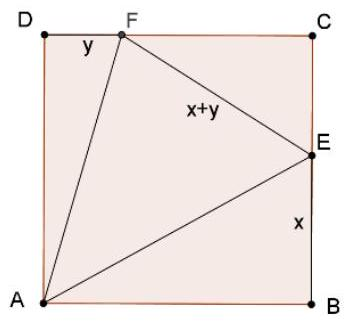
\includegraphics[max width=\textwidth, center]{2024_11_21_5666972ddc76bf3a54d6g-1}
  \item Pole powierzchni wielościanu opisanego na kuli o promieniu 1 wynosi 12 . Oblicz objętość tego wielościanu.
  \item Liczba rzeczywista \(x\) spełnia równanie \(x^{3}+4 x=8\). Znajdź wartość wyrażenia \(x^{7}+64 x^{2}\).
\end{enumerate}

\end{document}